\documentclass{article}
\usepackage{graphicx}
\usepackage{tikz}
\usepackage{pgfplots}
\pgfplotsset{compat=1.17}
\usepackage{hyperref}
\usepackage{tocloft}

\title{Reden-Export}
\date{\today}

\begin{document}

\maketitle

\tableofcontents

\section{ID2019201500}
\subsection{Rede: ID2019201500}
\subsubsection*{Tagesordnungspunkte:}
\subsubsection*{Redebeitrag}
Sehr geehrte Frau Präsidentin! Meine sehr geehrten Damen und Herren! Liebe Kolleginnen und Kollegen! Die \textbf{St.-Johannes-Bruderschaft Niederheide} aus der \textbf{Stadt Willich} in meinem Wahlkreis \textbf{Viersen} feiert in diesem Jahr ihr 100-jähriges Bestehen. Der Schützenverein aus dem kleinen Ort zwischen \textbf{Neersen} und \textbf{Schiefbahn} wurde ganz spontan in den ersten Stunden des Jahres 1924 gegründet. Nach einer gemeinsamen Silvesterfeier beschlossen seine Gründer: Unser Ort muss noch stärker zusammenhalten, und wir feiern ab jetzt \textbf{jedes Jahr} gemeinsam ein \textbf{Fest! – Gesagt}, getan: \textbf{Erntedank} 1924 war es so weit. Erstmals feierte der ganze Ort gemeinsam ein Schützenfest. \textbf{Einfach}, schnell und unbürokratisch – so gingen Vereinsgründung und Vereinsarbeit damals. \textbf{100 Jahre später ächzen Ehrenamt} und Vereine unter immer mehr Bürokratie. Ihre Mitglieder müssen sich mit \textbf{Papierkram} rumschlagen, statt sich für das Gemeinwohl zu engagieren. Immer weniger wollen aus Angst vor Fehlern und Haftung in \textbf{Vereinsvorständen} mitarbeiten. Die Organisation von Vereinsveranstaltungen gerät oft zum bürokratischen Hindernislauf. Ein Verein muss sich durchschnittlich 42 \textbf{Arbeitstage im Jahr}, also 6,5 Stunden pro Woche, um Zettelwirtschaft kümmern,  \textbf{Zeit}, die Ehrenamtlern nach Feierabend oder am Wochenende für ihre Familien und Freunde verloren geht; \textbf{Zeit}, die dafür fehlt, Kinder und Jugendliche für Sport zu begeistern, sich generationenübergreifend für Natur und Umwelt einzusetzen oder ein Mal im Jahr mit dem ganzen Ort auf der Karnevalssitzung oder im Schützenzelt zu feiern; \textbf{Zeit}, die viele davon abhält, sich überhaupt noch in Ehrenamt und Vereinen für unsere Gemeinschaft zu engagieren.  In den letzten Wochen und Monaten haben wir hier viel über Bürokratieabbau geredet. Vorschläge für weniger Bürokratie in Ehrenamt und Vereinen liegen längst auf dem Tisch. Rund 20 wurden allein in der Verbändeabfrage der Bundesregierung zum Bürokratieabbau gemacht. Auch der Nationale Normenkontrollrat hat ein einfacheres ehrenamtliches Engagement als zentrales Ziel für den Bürokratieabbau definiert und dafür konkrete Vorschläge präsentiert. Doch die Ampel hat all diese Vorschläge ungehört verhallen lassen. In ihrem \textbf{Bürokratieentlastungsgesetz} findet sich keine einzige Maßnahme, die Ehrenamt und Vereine von unnötiger Bürokratie befreit. Wer mit einem solchen Gesetz ein wenig Bürokratie für Aktiengesellschaften, für Steuerberater oder für Wirtschaftsprüfer abbaut, aber kein bisschen Bürokratie für Ehrenamt und Vereine, der wird der Bedeutung von Ehrenamt und Vereinen für unser demokratisches Gemeinwesen nicht gerecht.  Wir als \textcolor{red}{\textbf{CDU/CSU}} wollen das nicht hinnehmen. Ehrenamt und Vereine sind das Rückgrat unserer Gesellschaft. Sie sorgen im ganzen Land für Miteinander und Zusammenhalt. Sie haben deshalb unsere Anerkennung und Wertschätzung verdient, und zwar nicht nur in immer neuen Sonntagsreden, sondern auch, wenn es hier im \textbf{Deutschen Bundestag} ganz konkret darum geht, Engagement zu fördern, Ehrenamt zu stärken und Vereine zu entlasten.  Daher machen wir als \textbf{Union} heute auch ganz konkrete Vorschläge dafür: Wir wollen erstens die überbordende Bürokratie auch in der Ehrenamts- und Vereinsarbeit endlich systematisch bekämpfen. Wir setzen uns deshalb dafür ein, dass Bürokratiekosten im Ehrenamt um rund 25 Prozent sinken, dass künftig für jede neue Bürokratiebelastung im Ehrenamt doppelt so viel alte Bürokratie wegfällt und dass neue Regeln gemeinsam mit Vereinen und Ehrenamt auf ihre Praxistauglichkeit gecheckt werden. \textbf{Zweitens} wollen wir die Vereinsarbeit auch ganz konkret einfacher machen. Dafür wollen wir die leidigen Regelungen für Satzungs- und Vorstandsänderungen erleichtern, Haftungsrisiken für Vereinsvorstände und Vereinsmitglieder stärker begrenzen und Prüfungen bei der Gemeinnützigkeit und der \textbf{Steuer} vereinfachen. Drittens wollen wir Ehrenamt und Vereinsarbeit auch ganz konkret fördern. Die Anhebung der Ehrenamts- und der Übungsleiterpauschale ist längst überfällig. Wir wollen, dass Vereine ehrenamtliches Engagement ihrer Mitglieder künftig mit 1 200 Euro und ihre Ausbilder, Trainer und Übungsleiter mit 3 600 \textbf{Euro} honorieren können.  All diese Vorschläge machen das Ehrenamt nicht nur attraktiver; ein Verein muss sich nach ihrer Umsetzung auch durchschnittlich anderthalb Stunden pro Woche weniger, also rund 25 Prozent, um \textbf{Papierkram} kümmern. Und das ist nur der Anfang; denn mit unserem ambitionierten Ziel, weitere 25 \textbf{Prozent Bürokratie} im Ehrenamt abzubauen, wollen wir die Bürokratiebelastung perspektivisch sogar halbieren. Liebe Kolleginnen und Kollegen, es sind Vereine wie die \textbf{St.-Johannes-Bruderschaft Niederheide}, die darauf warten, dass wir ihnen das Leben wieder einfacher machen. Es sind Vereine wie die \textbf{St.-Johannes-Bruderschaft Niederheide}, die erwarten, dass wir ihre gewichtige Arbeit für uns alle auch durch konkrete Entscheidungen für mehr Attraktivität und weniger Bürokratie im Ehrenamt anerkennen und wertschätzen. Es sind Vereine wie die \textbf{St.-Johannes-Bruderschaft Niederheide}, die sich darauf verlassen können: Wir als \textcolor{red}{\textbf{CDU}} und \textcolor{red}{\textbf{CSU}} stehen fest an ihrer Seite, wenn es darum geht, Engagement zu fördern, Ehrenamt zu stärken und Vereine zu entlasten.  \section{Redner-Übersicht}
\begin{tabular}{ll}
Name: & Martin Plum \\
Partei: & CDU \\
Geburtsdatum: & Fri Feb 26 00:00:00 CET 1982 \\
Beruf: & Richter \\
\end{tabular}

\includegraphics[width=0.5\textwidth]{src/main/resources/pics/c0749b7cc401421662ae901ec8f9f660.jpg}\section{NLP-Daten-Übersicht}
\paragraph{POS-Statistiken:}
\begin{tabular}{ll}
\hline
POS-Tag & Häufigkeit \\ \hline
PWS & 1 \\ \hline
PTKVZ & 1 \\ \hline
VAINF & 1 \\ \hline
VVIZU & 2 \\ \hline
VMINF & 2 \\ \hline
PDAT & 3 \\ \hline
KOUI & 3 \\ \hline
PDS & 3 \\ \hline
TRUNC & 3 \\ \hline
KOKOM & 3 \\ \hline
PTKNEG & 4 \\ \hline
PIS & 5 \\ \hline
PRELS & 6 \\ \hline
PRF & 8 \\ \hline
KOUS & 8 \\ \hline
VMFIN & 9 \\ \hline
NE & 10 \\ \hline
PTKZU & 10 \\ \hline
VVPP & 11 \\ \hline
APPRART & 12 \\ \hline
PIAT & 13 \\ \hline
PROAV & 13 \\ \hline
VAFIN & 14 \\ \hline
CARD & 14 \\ \hline
PPOSAT & 19 \\ \hline
VVFIN & 24 \\ \hline
PPER & 25 \\ \hline
VVINF & 29 \\ \hline
ADJD & 33 \\ \hline
ADJA & 36 \\ \hline
ART & 46 \\ \hline
ADV & 48 \\ \hline
KON & 48 \\ \hline
APPR & 63 \\ \hline
NN & 183 \\ \hline
\end{tabular}

\paragraph{Stimmung:}
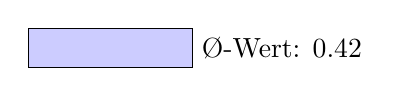
\begin{tikzpicture}
\draw[fill=blue!20] (0,0) rectangle (2.0820000000000003,0.5);
\node[anchor=west] at (2.0820000000000003,0.25) {Ø-Wert: 0.42};
\end{tikzpicture}

\begin{itemize}
\item {\textbf{Positivster Text}: \\ 

Sie haben deshalb unsere Anerkennung und Wertschätzung verdient, und zwar nicht nur in immer neuen Sonntagsreden, sondern auch, wenn es hier im Deutschen Bundestag ganz konkret darum geht, Engagement zu fördern, Ehrenamt zu stärken und Vereine zu entlasten.   (0.97)};
\item {\textbf{Negativster Text}: \\ 

Immer weniger wollen aus Angst vor Fehlern und Haftung in Vereinsvorständen mitarbeiten. (-0.68)};
\end{itemize}

\clearpage
\paragraph{Topics:}
\begin{longtable}{ll}
\hline
Topic & Score \\ \hline
\endfirsthead
\hline
Topic & Score \\ \hline
\endhead
\hline
\multicolumn{2}{r}{\textit{Fortsetzung auf nächster Seite}} \\ \hline
\endfoot
\hline
\endlastfoot
\textbf{1663 - 1746 Government} & \textbf{1.00} \\ \hline
\textbf{1835 - 1928 Government} & \textbf{1.00} \\ \hline
\textbf{3971 - 4142 Social} & \textbf{1.00} \\ \hline
3890 - 3970 Social & 1.00 \\ \hline
4947 - 5182 Social & 1.00 \\ \hline
3579 - 3815 Social & 1.00 \\ \hline
1548 - 1663 Social & 1.00 \\ \hline
2759 - 3018 Social & 1.00 \\ \hline
3816 - 3889 Social & 1.00 \\ \hline
2638 - 2698 Social & 1.00 \\ \hline
2175 - 2306 Government & 1.00 \\ \hline
1929 - 2107 Government & 0.99 \\ \hline
4703 - 4946 Social & 0.99 \\ \hline
3018 - 3207 Social & 0.99 \\ \hline
3505 - 3578 Social & 0.99 \\ \hline
1317 - 1547 Social & 0.99 \\ \hline
2108 - 2174 Transportation & 0.98 \\ \hline
1094 - 1316 Social & 0.98 \\ \hline
446 - 592 Government & 0.96 \\ \hline
4142 - 4205 Social & 0.95 \\ \hline
4539 - 4702 Social & 0.86 \\ \hline
4381 - 4538 Government & 0.83 \\ \hline
2594 - 2637 Government & 0.83 \\ \hline
0 - 30 Government & 0.82 \\ \hline
2699 - 2758 Civil & 0.80 \\ \hline
101 - 184 Civil & 0.79 \\ \hline
816 - 916 Social & 0.75 \\ \hline
4206 - 4352 Government & 0.71 \\ \hline
3208 - 3504 Social & 0.68 \\ \hline
69 - 100 Government & 0.68 \\ \hline
185 - 241 Government & 0.67 \\ \hline
1747 - 1834 Social & 0.66 \\ \hline
593 - 651 Government & 0.65 \\ \hline
1006 - 1093 Social & 0.65 \\ \hline
242 - 380 Social & 0.61 \\ \hline
4353 - 4380 Government & 0.59 \\ \hline
742 - 815 Social & 0.58 \\ \hline
652 - 741 Social & 0.57 \\ \hline
2307 - 2594 Government & 0.54 \\ \hline
917 - 1005 Social & 0.49 \\ \hline
31 - 68 Government & 0.48 \\ \hline
381 - 445 Law & 0.44 \\ \hline
652 - 741 Government & 0.42 \\ \hline
742 - 815 Government & 0.41 \\ \hline
381 - 445 Government & 0.34 \\ \hline
242 - 380 Domestic & 0.34 \\ \hline
1747 - 1834 Government & 0.33 \\ \hline
1006 - 1093 Government & 0.32 \\ \hline
2307 - 2594 Social & 0.31 \\ \hline
3208 - 3504 Government & 0.30 \\ \hline
4206 - 4352 Social & 0.26 \\ \hline
917 - 1005 Government & 0.22 \\ \hline
816 - 916 Government & 0.20 \\ \hline
593 - 651 Social & 0.20 \\ \hline
917 - 1005 Domestic & 0.18 \\ \hline
4381 - 4538 Social & 0.16 \\ \hline
69 - 100 Social & 0.15 \\ \hline
185 - 241 Domestic & 0.13 \\ \hline
2307 - 2594 Domestic & 0.12 \\ \hline
0 - 30 Social & 0.12 \\ \hline
381 - 445 Social & 0.11 \\ \hline
4353 - 4380 International & 0.11 \\ \hline
31 - 68 Domestic & 0.10 \\ \hline
4353 - 4380 Law & 0.10 \\ \hline
31 - 68 Social & 0.09 \\ \hline
2699 - 2758 Government & 0.09 \\ \hline
31 - 68 Civil & 0.09 \\ \hline
69 - 100 Civil & 0.09 \\ \hline
4539 - 4702 Civil & 0.07 \\ \hline
101 - 184 Social & 0.06 \\ \hline
31 - 68 Macroeconomics & 0.06 \\ \hline
917 - 1005 Labor & 0.06 \\ \hline
4353 - 4380 Macroeconomics & 0.06 \\ \hline
185 - 241 Macroeconomics & 0.05 \\ \hline
2594 - 2637 Civil & 0.05 \\ \hline
101 - 184 Government & 0.04 \\ \hline
185 - 241 Social & 0.04 \\ \hline
4142 - 4205 Labor & 0.04 \\ \hline
2699 - 2758 Social & 0.04 \\ \hline
185 - 241 Law & 0.04 \\ \hline
816 - 916 Civil & 0.04 \\ \hline
593 - 651 Domestic & 0.04 \\ \hline
593 - 651 Law & 0.04 \\ \hline
4539 - 4702 Law & 0.03 \\ \hline
593 - 651 Civil & 0.03 \\ \hline
2594 - 2637 Macroeconomics & 0.03 \\ \hline
4353 - 4380 Civil & 0.03 \\ \hline
381 - 445 Domestic & 0.03 \\ \hline
4206 - 4352 Labor & 0.02 \\ \hline
31 - 68 Law & 0.02 \\ \hline
185 - 241 Culture & 0.02 \\ \hline
31 - 68 Environment & 0.02 \\ \hline
2699 - 2758 Law & 0.02 \\ \hline
101 - 184 Law & 0.02 \\ \hline
917 - 1005 Law & 0.02 \\ \hline
1094 - 1316 Labor & 0.02 \\ \hline
31 - 68 Defense & 0.02 \\ \hline
69 - 100 Domestic & 0.02 \\ \hline
242 - 380 Law & 0.02 \\ \hline
381 - 445 Macroeconomics & 0.02 \\ \hline
381 - 445 Civil & 0.02 \\ \hline
2594 - 2637 Social & 0.02 \\ \hline
101 - 184 Immigration & 0.01 \\ \hline
4353 - 4380 Technology & 0.01 \\ \hline
2699 - 2758 International & 0.01 \\ \hline
31 - 68 Transportation & 0.01 \\ \hline
31 - 68 Housing & 0.01 \\ \hline
31 - 68 International & 0.01 \\ \hline
381 - 445 Health & 0.01 \\ \hline
4353 - 4380 Education & 0.01 \\ \hline
101 - 184 International & 0.01 \\ \hline
2594 - 2637 International & 0.01 \\ \hline
4353 - 4380 Social & 0.01 \\ \hline
101 - 184 Culture & 0.01 \\ \hline
242 - 380 Government & 0.01 \\ \hline
2108 - 2174 Government & 0.01 \\ \hline
4353 - 4380 Transportation & 0.01 \\ \hline
101 - 184 Agriculture & 0.01 \\ \hline
31 - 68 Culture & 0.01 \\ \hline
2594 - 2637 Domestic & 0.01 \\ \hline
0 - 30 Civil & 0.01 \\ \hline
69 - 100 Law & 0.01 \\ \hline
242 - 380 Civil & 0.01 \\ \hline
\end{tabular}
}

\end{document}